\section{Tests realisés pour valider le fonctionnement du TP}
\bframe{
    Les tests réalisés ont simplement été de \quo{jouer au jeu}, avec un ou plusieurs clients, 
    la procédure attendu étant assez guidé l'étendu de panel de test à réaliser en est moindre. 
    
    Cependant elle en demeure non trivial du à l'échange d'informations via un serveur.
    Pour vérifier si les sockets sont bien fermées on peut utiliser la commande \code{ss -tn}\\
    \code{man ss} affiche: \\
    \quo{\textit{\code{ss} is used to dump socket statistics. It allows showing information similar to netstat.  It can display more TCP and state information than other tools.} \\
    $\ $ \code{-t}: Display TCP sockets. \\
    $\ $ \code{-n}: Do not try to resolve service names. Show exact bandwidth values, instead of human-readable.} \\
    
    
    \vspace{0.3cm}
    
    Voir le screenshot ci-après pour plus de détail sur les tests.
}

\bframe{
\vspace{-0.2cm}
\begin{figure}[H]
    \centering
    %\hspace{-0.45cm}    
    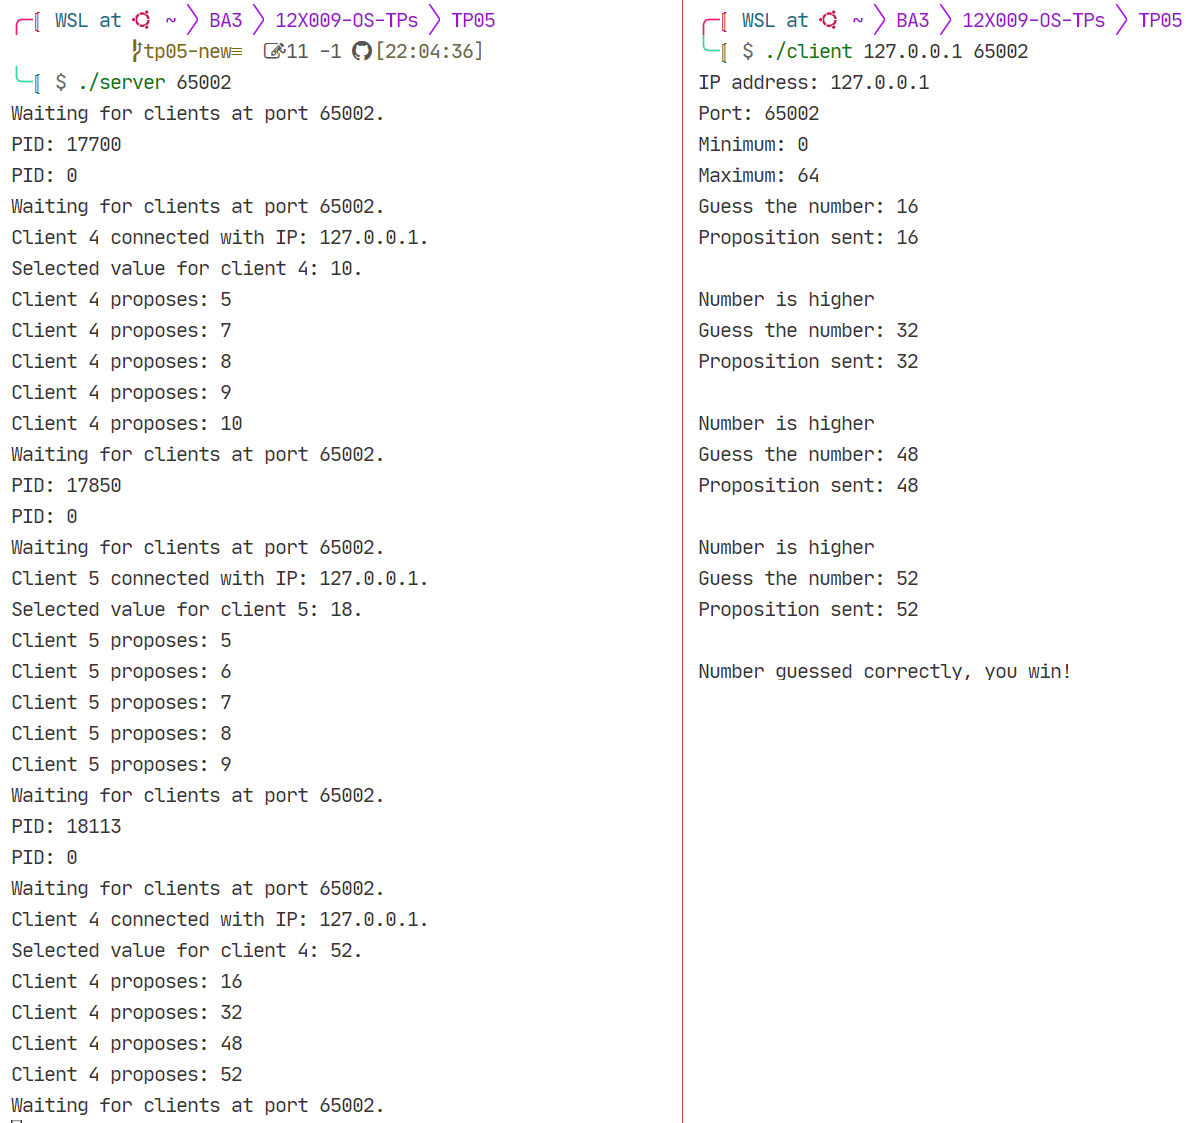
\includegraphics[width=10.5cm, height=8.2cm]{images/test-tp5-01.png}
    \caption{Test de l'implémentation du TP05.\label{fig:Figure1}}
    \end{figure}
    \unskip
}